\chapter{分析手法}
\label{chap:method}
\fancyhf{}
\rhead{\thepage}
\lhead{第\ref{chap:method}章 分析手法}
\cfoot{\thepage}
本章では,
分析手法について説明する.

まず,分析手法全体の流れを概説し,手法全体が3つの要素から構成されることを述べたのち,
各要素について詳述する.

\vvspace


\section{分析手法全体の流れ}
まず,分析手法全体の流れを説明する.
%本研究の手法は,データセットの作成,問題空間を知識タグ空間に変換する写像行列の学習,知識タグの抽出と検証の3つの要素から構成される.
本研究の手法は,データセットの作成という事前処理と,
%知識分類の学習,知識分類の性能検証,知識分類の性質分析
提案手法による知識分類の学習,
学習された知識分類の知識獲得予測性能に関する検証,
学習された知識分類の性質に関する比較分析
という3つの分析から構成される.


まず,データセットの作成について述べる.
本論文が扱う,生徒の知識獲得予測において,
生徒が知識を獲得しているか否かの評価には,生徒の問題回答ログデータを対象データセットとして用いる.
その際,比較検証に用いるため,
知識獲得の予測に利用できる複数のデータセットを利用し,また,本研究に適用するために,幾つかの条件に基づいて対象データを抽出する.


次に,3つの分析の手法について述べる.

まず,知識分類の学習について述べる.
知識獲得の予測性を最適化するような知識分類を抽出するには,
問題の空間と,抽出目的の知識タグ空間の最適な関係性を深層学習によって学習する必要がある.
そのために,問題を知識分類に変換する写像関数をパラメータ化し,回答正誤予測の最適化の過程で同時に学習する.
このモデル構造は,Deep Knowledge Tracingのモデルを拡張して設計する.
学習された写像関数は連続値表現の行列として表されており,
これを適切に離散化することで,知識分類を抽出する.

次に,知識分類の性能検証について述べる.
学習された知識分類に基づき,問題を知識タグ変換し,知識獲得予測を行う.
抽出された知識タグを用いることにより,既存の知識タグや一般的な次元圧縮手法によって得た知識タグを用いる場合より,
高い精度で知識獲得が予測できることを示すことで,
本手法により知識獲得の予測性を最適化する知識分類が得られたことを定量的に示す.

最後に,知識分類の性質分析について述べる.
学習された知識分類に基づく知識タグの性質や構造を,既存の知識タグの構造と比較することにより,その性質を定性的に検証する.


以上の分析手法全体の流れを,図\ref{fig:workflow}にまとめた.
\begin{figure}[htb]
\begin{center}
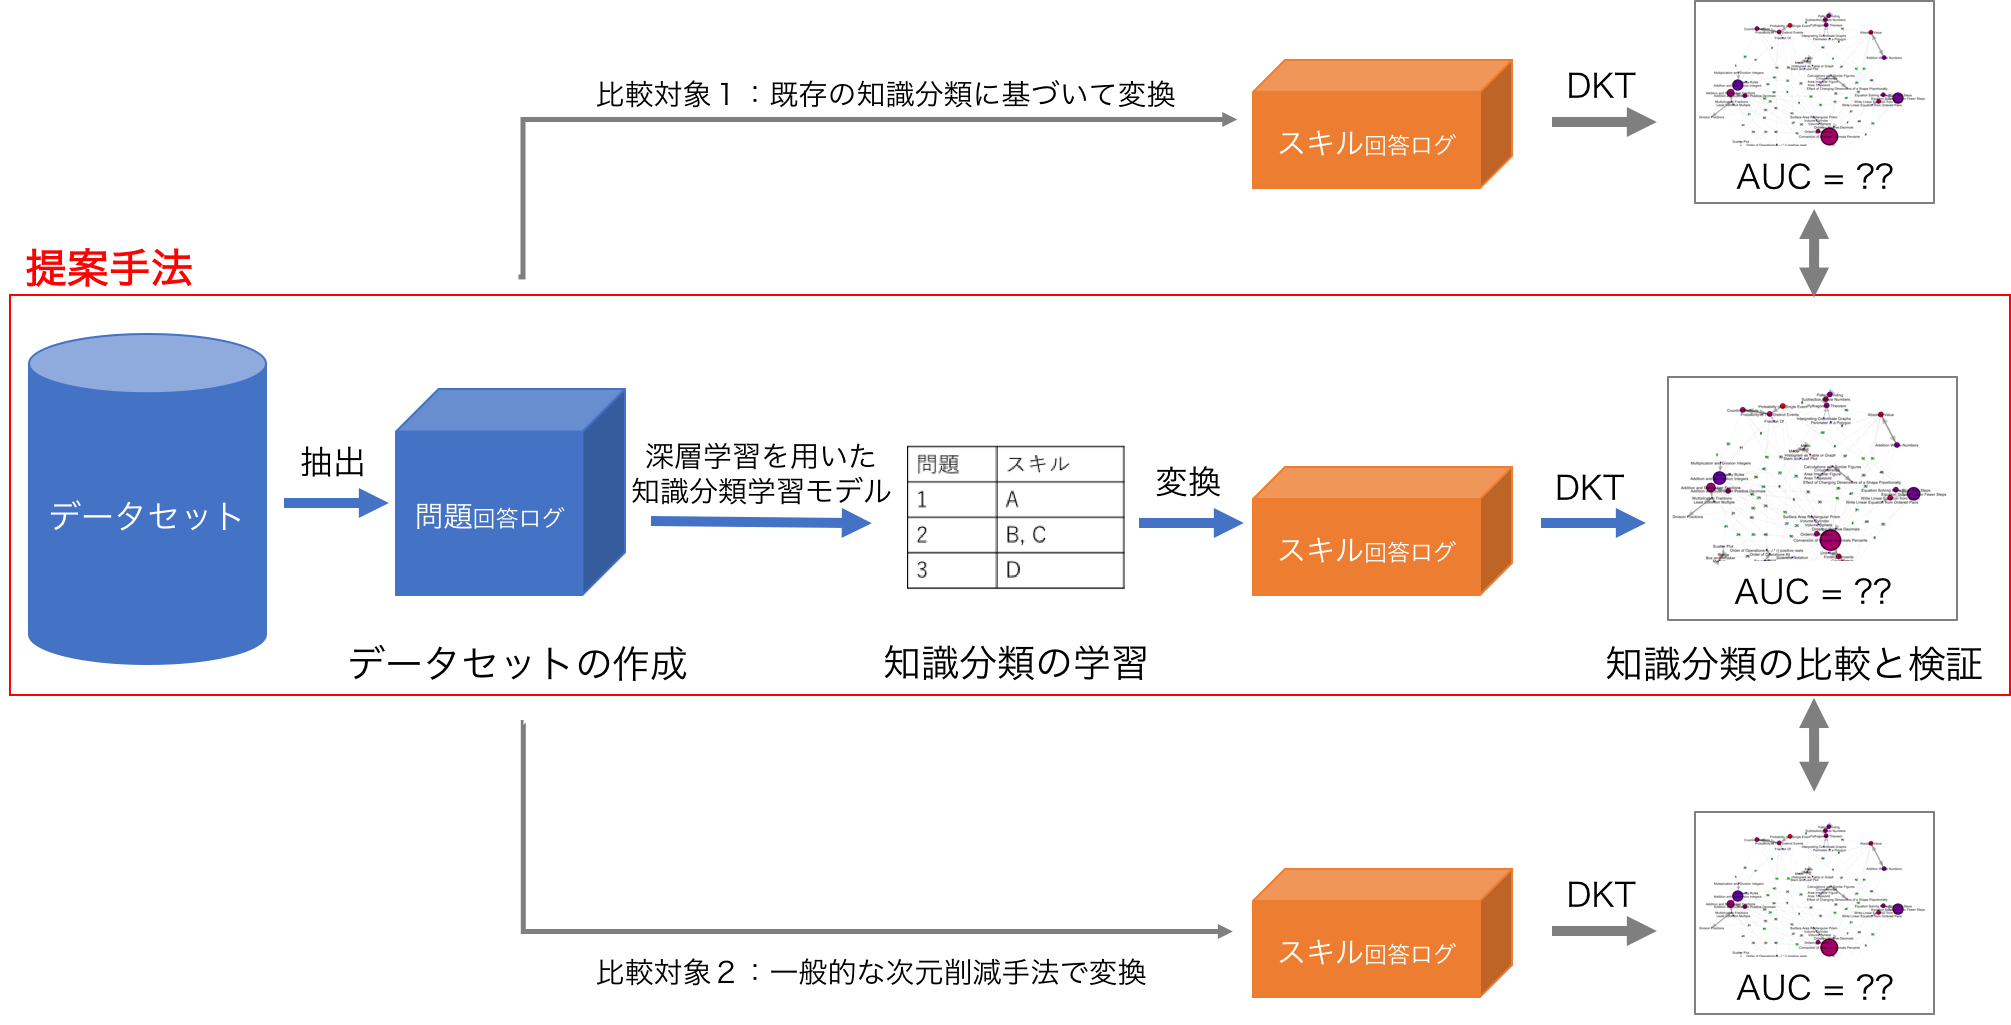
\includegraphics[width=400pt]{./img/workflow.png}
\end{center}
\caption{分析手法全体の流れ}
\label{fig:workflow}
\end{figure}

以降では,
データセットの作成,
提案手法による知識分類の学習,
学習された知識分類の知識獲得予測性能に関する検証,
学習された知識分類の性質に関する比較分析
について順に詳述する.


\section{データセットの作成}
本論文が扱う生徒の知識獲得予測においては,
生徒の問題回答ログデータをデータセットとして用いる.
生徒の問題への回答結果は,その問題が問う知識を,生徒が既に獲得しているか否かを表現していると捉えることができるため,
回答結果が正解であれば,該当の知識を既に獲得しており,
回答結果が不正解であれば,該当の知識を未だ獲得していないと捉えることができるからである.

問題回答ログデータから作成するデータセットは,下記の要件を満たす必要がある.
\begin{enumerate}
	\item データセットが大規模であること.
	\item 比較検証できるデータセットが複数存在すること.
	\item 問題に既存の知識タグが割り当てられていること.
\end{enumerate}


まず,データセットが大規模である必要について説明する.
一般に,深層学習は大量のデータを元に特徴的な表現を抽出するため,
深層学習モデルを十分に学習させるには,大規模なデータが必要である.
これは,深層学習モデルの一つであるRecurrent Neural Network(RNN)を活用するDeep Knowledge Tracingについても同様である\cite{piech2015deep}.
したがって,大規模なデータを有することがデータセットの要件の一つとなる.

また,深層学習によって知識獲得の予測を行う本研究においては,単に全体のデータ数が多いだけでなく,
分析対象となる個別の問題や生徒について,十分なデータ数を確保できることが重要である.
例えば,一度しか回答されていない問題については,
その問題の正答や誤答によって,生徒の知識状態がどのように変化するかが観察できないため,分析に適していない.
また,十分な数の生徒のデータがないと,特定の生徒の学習傾向が強く反映され,
知識獲得過程の一般性が損なわれる可能性がある.


次に,比較検証できるデータセットが複数存在する必要について説明する.
本研究で用いる,問題回答ログからなるデータセットは,
そのデータセットが提供されるプラットフォームにより,問題を回答している集団や,扱っている教科,内容のレベルなどが異なる.
特定のデータセットのみに対して得られた結果は,そのデータセットの環境においてのみ有効である可能性があり,
一般性のある結果や知見が得られたとは言いにくい.
そのため,本研究では,教科を数学に絞った上で,複数のプラットフォームにおける問題回答ログから複数のデータセットを作成することで,
手法の一般性を検証する.
なお,数学に限らない,他教科への適用可能性については,第6章で考察する.


最後に,回答された問題に,既存の知識タグが割り当てられている必要について説明する.
本研究では.現在の一般的な知識獲得予測に用いられている知識タグは,
人間の複雑な知識獲得過程を表現する上では最適化されていない,という仮定に立ち,
問題回答ログのみを利用して,より最適化された知識タグを作成することを目的としている.
抽出された知識タグの妥当性を検証するには,既存の知識タグと比較することが必要であり,
そのため,分析対象となるデータセットは,問題に既存の知識タグが割り当てられている必要がある.









\section{提案手法による知識分類の学習}
本節では,知識分類学習モデルによる知識分類の学習について述べる.

本研究では,
知識獲得予測を最適化する知識分類を学習するために,
問題を知識分類に変換する関数をパラメータ化し,Knoeledge Tracingの最適化の過程で同時に学習する.
なお,以降では,この提案手法のモデル構造を「知識分類学習モデル」と呼ぶ.
この知識分類学習モデルの構造は,Deep Knowledge Tracing(以下,DKT)を元に設計されているため,
まず,DKTを拡張する方法について述べる.

その後,抽出された問題空間を知識タグ空間に写像する関数を離散化し,実際の知識分類を作成する方法について述べる.


\subsection{DKTの拡張による写像関数の学習}
\label{sec:tag_learn}

問題を知識分類に変換する写像関数をパラメータ化し,Knoeledge Tracingの最適化の過程で同時に学習するために,
既存のDKTモデルを拡張する方法を,以下の3つの要素に分けて説明する.

\begin{enumerate}
	\item 入力データの粒度
	\item モデル全体の構造
	\item 最適化手法
\end{enumerate}


\subsubsection{入力データの粒度}
まず,既存のDKTと大きく異なる点として,モデルに入力されるデータの粒度の違いについて述べる.
DKTのモデルにおいては,使用するデータの元は生徒の問題回答ログデータであるが,
モデルへの入力は,事前に定義された知識分類に基づいて,知識タグに落とし込まれ,どの知識タグに回答したかが入力される.
これは,既存の知識タグの中で,生徒がどのように知識獲得をしていくかを予測することを前提にしているためであるが,
本研究においては,そもそもの問題と知識タグの関係性を最適化することを目的とするため,この入力は適さない.

よって本研究では,モデルへの入力は問題に対する回答のままにとどめ,
生徒が次にどの問題に正解するかを予測する過程において,
深層学習モデル自身に最適な知識の分類方法を判断させることで,
最終的に,知識獲得予測を最適化するような知識分類を学習させる.

こうして学習された知識分類に基づく知識タグは,結果的に知識獲得の文脈で最適化されていると考えることができ,
既存の知識タグと比較することで,その性質を解釈することができる.


\subsubsection{モデル全体の構造}
次に,具体的なモデル全体の構造の拡張について述べる.
まず,
DKTでは入力がRNNの隠れ層へ直接伝達されるのに対し,
知識分類学習モデルは,
まず入力層の問題空間$X$から,抽出目的の知識タグ空間$U$への写像を行う.
ここで言う知識タグ空間とは,既存の知識タグと同じ次元数に設定された空間で,
問題回答の正誤の情報を低次元の空間で表すことを目的としている.

具体的には,
まず,問題数を$M$とした場合,モデルへの入力ベクトル${\bf x}_t$の長さは$2M$である.
抽出目的の知識タグの次元数は,既存の知識タグと同じ次元数に揃え,事前に$N$と定義する.
そして,$M$次元の問題空間$X$から$N$次元の知識タグ空間$U$へ変換する写像関数$P$を,以下の式により定義する.
\begin{eqnarray}
{\bf P} = \sigma( {\bf W}_{xu} {\bf x} + {\bf b}_u)
\end{eqnarray}
ここで,
${\bf x}$は長さ$M$の問題空間ベクトルを指し,
${\bf W}_{xu}$は$MxN$の大きさの重み行列を指し,
${\bf b}_u$は長さ$N$のバイアス項を指し,
$\sigma$は$1 / (1 + e^{-x})$で定義されるシグモイド関数を指す.
訓練時には,${\bf W}_{xu}$,${\bf b}_u$を学習する.
\begin{eqnarray}
\label{eq:encode}
{\bf P} = \sigma( {\bf W}_{xu} {\bf x} + {\bf b}_u)
\end{eqnarray}

時刻$t$における問題の回答の正誤の情報は,DKT同様,それぞれ長さ$M$のベクトルで別々に表現し,連結して長さ$2M$のベクトル${\bf x}_t$として表現されている.
写像関数$P$を,${\bf x}_t$の前半の正答部分と後半の誤答部分に別々に適用し,連結することによって,
回答の正誤の情報を保った,
長さ$2N$の知識タグ空間ベクトル${\bf u}_t$が生成できる.
\begin{eqnarray}
{\bf u}_t = [{\bf P}({\bf x}_{t_positive}), {\bf P}({\bf x}_{t_negative})]
\end{eqnarray}
ここで,${\bf x}_{t_positive)}$,${\bf x}_{t_negative})$はそれぞれ問題回答の正答と誤答を表す長さ$M$のベクトルである.

こうして得られた知識タグ空間ベクトル${\bf u}_t$は,
一般的なRNN同様,隠れ層を経由して時系列情報を反映した後,再び長さ$2N$の知識タグ空間ベクトル${\bf v}_t$となる.
\begin{eqnarray}
{\bf h}_t &=& \tanh({\bf W}_{uh} {\bf u}_t + {\bf W}_{hh}  {\bf h}_{t-1} + {\bf b}_h)\\
{\bf v}_t &=& \sigma( {\bf W}_{hv} {\bf h}_t + {\bf b}_v)
\end{eqnarray}
ここで,
${\bf h}_t$は時刻$t$の隠れ層を指し,
${\bf W}_{uh}$,${\bf W}_{hh}$はそれぞれ重み行列を指し,
${\bf b}_h$,${\bf b}_v$はそれぞれバイアス項を指し,
$\tanh$は$( e^x - e^{-x} )/( e^x + e^{-x} )$で定義されるHyperbolic Tangent関数を指す.
この知識タグ空間ベクトル${\bf v}_t$は,時刻$t$までの回答情報を反映した,生徒の知識タグ空間における知識状態を表していると言える.

最終的に,この知識タグ空間ベクトル${\bf v}_t$から,予測結果として$M$次元の問題回答予測ベクトル${\bf y}_t$を算出する.
\begin{eqnarray}
{\bf y}_t &=& \sigma( {\bf W}_{vy} {\bf v}_t + {\bf b}_y)
\end{eqnarray}
ここで,
${\bf W}_{vy}$は重み行列を指し,
${\bf b}_y$はバイアス項を指す.

${\bf y}_t$は0から1の間の値を取り,次の時刻$t+1$において各問題に正答する確率を表しており,
既存のDKTと同じ予測表現となっている.

%ここで,問題空間から知識タグ空間への符号化は,正答ベクトルと誤答ベクトルにそれぞれに同じ写像関数を適用していたのに対し,
%知識タグ空間から問題空間への復号化は,正答ベクトルと誤答ベクトルで区別せず,まとめて1つの写像関数が適用されていることに注意されたい.
%これは,問題空間から知識タグ空間への符号化は,その時点でどの問題に正答・誤答したかを元に,単純な関係性に基づいて写像を行うが,
%知識タグ空間ベクトルから,次の時刻における問題の回答正誤を予測するには,
%それまでの時刻の回答情報を反映した,知識タグ空間における正答・誤答を総合して正解確率を予測する必要があり,
%そのため,まとめて一つの写像関数を適用している.

\begin{figure}[htb]
\begin{center}
	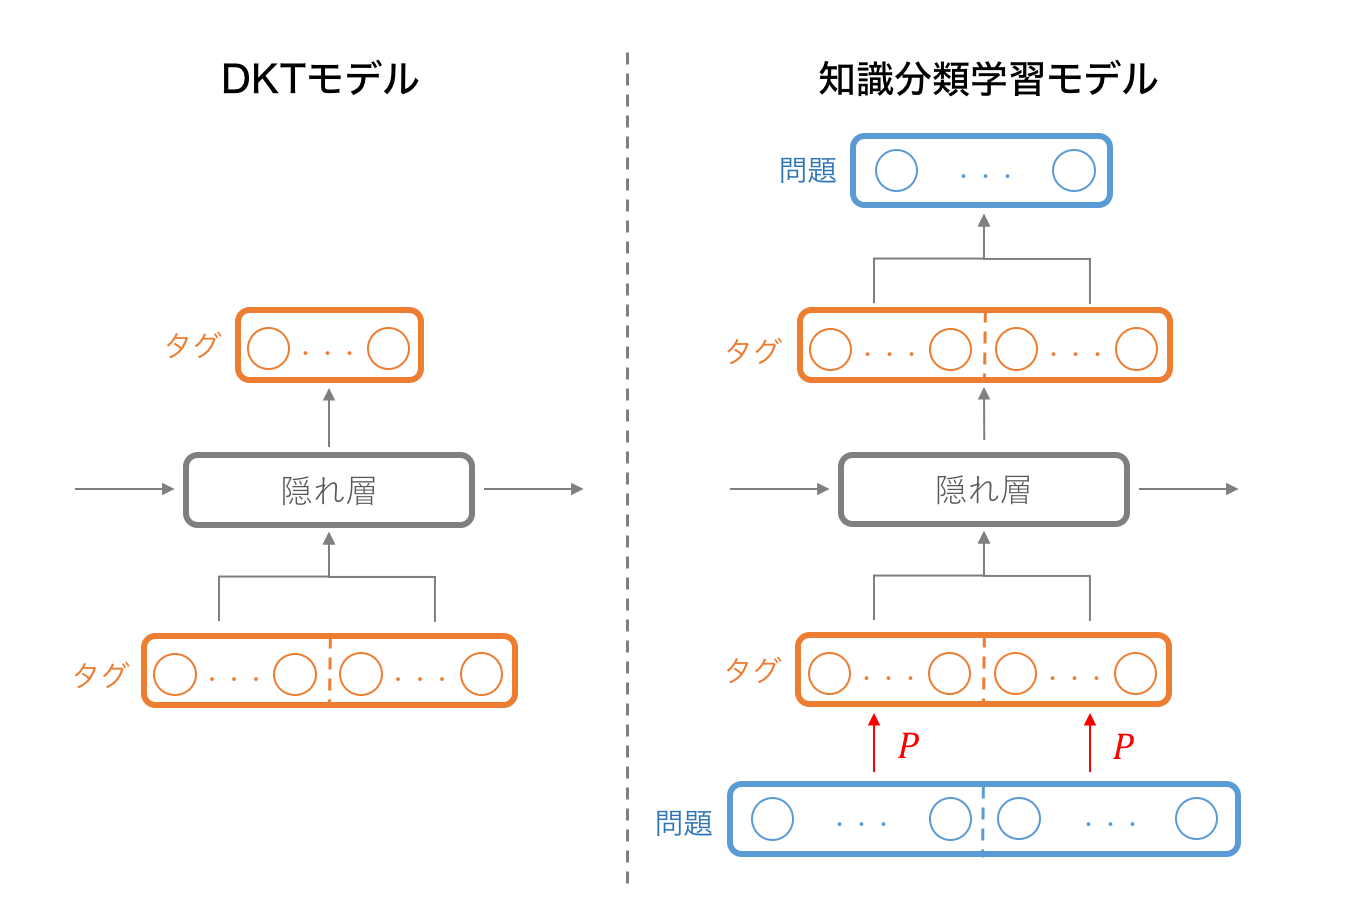
\includegraphics[width=360pt]{./img/model.png}
	\caption{モデル構造上の拡張}
	%\caption{モデル構造上の拡張 \protect \footenotemark}
	\label{fig:model}
\end{center}
\end{figure}
%\footnotetext{
%問題空間からタグ空間への写像関数$P$は$P=\sigma({\bf W} x + b)$で表され.正答部分と誤答部分に同じ関数が適用される.
%}

以上のようなモデル構造上の拡張をまとめた図を図\ref{fig:model}に表す.
橙色の層はタグ空間を,青色の層は問題空間を表し,層が二つに区切られている部分は前半・後半がそれぞれ正答・誤答の情報を表現している.
問題空間からタグ空間への写像関数$P$は$P=\sigma({\bf W} x + b)$で表され.正答部分と誤答部分に同じ関数が適用される.

この拡張の目的は,
知識獲得予測の最適化を行う過程で,
$M$次元の問題空間$X$から$N$次元の知識タグ空間$U$へ変換する写像関数$P$をパラメータ化し,学習することにある.



\subsubsection{最適化手法}
既存のDKTにおける最適化手法は,
次の時刻の問題回答予測ベクトルと,実際の次の時刻の問題回答ベクトルの誤差を最適化手法として,これを最小化するものである.
\begin{eqnarray}
\label{eq:log_sum}
{\log(p_1 \times p_2 \times \dots \times p_{m_t}) = \sum_{k}^{m_t} \log(p_k)}
\end{eqnarray}
であるため,
${\bf\tilde{ \delta}}({\bf q}_{t+1})$を時刻$t+1$にどの問題が回答されたかの$m_t$-hotベクトルとし,
${\bf a}_{t+1}$を時刻$t+1$に対応する問題で正答したか否か($1$か$0$)のベクトルとすれば,
損失関数は
\begin{eqnarray}
\label{eq:prediction_entropy}
{L_p = \sum_t l({\bf y}_t^T {\bf \tilde{\delta}}({\bf q}_{t+1}), {\bf a}_{t+1})}
\end{eqnarray}
である.
この損失関数を,問題回答予測に関する損失関数$L_p$とする.


本研究では,この問題回答予測に関する損失関数に加え,
式\ref{eq:autoencoder_hidden}--\ref{eq:autoencoder_loss}で表される再構成誤差も損失関数として導入する.
ここで,式\ref{eq:autoencoder_hidden,eq:autoencoder_reconstruct}におけるパラメータについては,
本研究では,
${\bf W}$,${\bf b}$が,
入力層で問題空間から知識タグ空間へ写像する際に用いる
${\bf W_{xu}}$,${\bf b_u}$
であり,
${\bf W'}$,${\bf b'}$が,
出力層で知識タグ空間から問題空間へ復元する際に用いる
${\bf W_{vy}}$,${\bf b_y}$
である.

この入力の再構成誤差の損失関数を$L_r$とすると,
結果的に,
モデル全体の損失関数$L$は以下の式によって定められ,
この損失関数を最小化するようにモデルが学習される.
\begin{eqnarray}
\label{eq:total_loss}
{L = L_p + L_r}
\end{eqnarray}


ここで,再構成誤差を損失関数に導入する理由について述べる.
まず,一般的に再構成誤差を用いるAutoencoderは,
深層学習モデルに良い初期値を与えるための事前学習のための仕組みとして用いられるが,
本研究では,このAutoencoderの構造を,DKTと同時に学習させるモデル構造になっている.

Autoencoderの構造を,事前学習ではなく普通の学習モデルに適用することは,
必ずしも精度向上につながるわけではないため,一般的ではなく,
単純に低次元のベクトルへ埋め込むのみに留まることが多い.

本研究では,
問題から知識分類を学習するには十分とはいえないデータ量が,一部の問題について存在するため,
データの特徴を把握しきれないunderfittingの状況に陥る可能性がある.
そうした学習不足への対策として,学習を矯正する正則化項として再構成誤差を導入している.
このように,データ数が不足する場合に,モデルがより適切に学習を進めるように正則化項を設ける手法は一般的であり,
有効な手法とされている.

また,こうした問題と知識タグにAutoencoderの関係を定義することは,
問題の正答・誤答と知識タグの理解状態は,相互に変換できるはずだという,
教育学的な文脈との整合性と合致し,
学習される知識分類の質を損ねないと判断した.


\subsection{写像関数の離散化による知識分類の作成}
\ref{sec:tag_learn}の知識分類学習モデルで得られた写像関数$P$から,
実際に知識分類を作成して問題をタグ付けし,既存の知識タグと比較する手法について説明する.


知識獲得予測の最適化の過程で得られた写像関数$P$は,
$M$次元の問題空間を$N$次元の知識タグ空間に写像する,$MxN$の大きさの行列として表現されている.
この行列は0から1の値を取る連続値表現であるため,そのままでは問題がどの知識タグに紐づくかを特定することはできない.
そのため,何らかの方法で,この行列を0か1の2値を取る離散表現に改める必要がある.

離散化の方法としては,各問題に対して最も関係性の強い知識タグのみをタグとする方法や,
行列全体で特定の閾値を定め,その閾値を超えたものをタグとする方法,両者を組み合わせる方法など,
様々な方法が考えられる.
各方法によって,抽出された知識タグの性質の異なる解釈をすることが可能だが,
本研究では,知識獲得予測に適用した際に最も良い精度で予測できる分類を,
知識獲得の遷移を最もよく説明する分類として見なして利用し,その性質も解釈する.









\section{学習された知識分類の知識獲得予測性能に関する検証}
次に,
抽出された知識タグ(以下,抽出タグ)の知識獲得予測における性能を,比較検証する手法について述べる.
まず,抽出タグが,知識獲得の予測性を最適化する分類になっていることを示すために,
抽出タグに基づいた回答ベクトルを一般的なDKTに入力することで,
既存の知識タグ(以下,既存タグ)を用いた場合よりも精度が向上することを確認する.
また,この精度向上が,知識獲得予測の最適化の過程で知識分類を作成したことに起因することを示すため,
PCAやAuto Encoderといった,知識獲得予測を用いない一般的な次元圧縮手法で作成した知識タグを用いた場合とも比較を行う.

これは,本手法における知識分類の作成が,
\begin{itemize}
	\item 人間の可読性を目的として専門家によって設計された分類か否か
	\item 知識獲得予測の文脈で最適化された分類か否か
\end{itemize}
という二つの観点において,既存の知識分類と異なることを受け,
性能の変化が何に起因してもたらされたのかという,差分をより明確にするために行う検証である.





\section{学習された知識分類の性質に関する比較分析}
最後に,こうした知識獲得予測の精度向上という定量的な検証に加え,
抽出タグの性質について,既存の知識タグとの比較を通して,定性的な分析も行う.
これは,知識獲得予測において最適化されている知識分類の性質を解釈し,新たな知見を得ることで,
教育における実用性を考察することにつなげることが目的である.

まず,抽出タグと,既存の知識タグについて,
回答される頻度や問題との紐付き方の分布に着目し,
知識獲得予測の精度を向上させる要因を,データの構造から分析する.

また,抽出タグと既存の知識タグが,
内容の面においてどのような関係性があり,
既存の知識タグがどのように再配置されたのかを検証する.

抽出タグと既存タグの内容を比較する方法として,まず,
抽出タグが紐づく問題と,既存タグが紐づく問題から,
抽出タグと既存タグの共起行列を作成する.
この行列は,各抽出タグを,各既存タグとの関係性の近さを表現している行列と捉えることができるが,
各抽出タグの特徴をより明確に捉えるために,TF-IDF法[参考文献引用or前提知識]を用いて,特徴の重み付けを行う.
TF-IDF法は,元々文書の分類に用いられる手法で,
複数の文書がある時に,各文書を特徴づける単語を特定することを目的にしている.
具体的には,まず,各文書内での,各単語の出現頻度(Term Frequency,以下TF)を求める.
TFは,文書内に多く出現する単語ほど重要だ,という考えに基づいた指標であるが,
TFのみだと,例えば助詞や助動詞と言った,いくつもの文書で横断的に使われている単語の重要度が高くなってしまうため,
各単語が全文書の内いくつの文書にあらわれているかという制約(Inverse Document Frequency)を設けて,
一般的な単語の影響を除外する.
単語$i,j$のTF,IDFと,それらを用いたTF-IDF値は以下の式で表される.
\begin{eqnarray}
TF_{i,j} &=& \frac {n_{i,j}}{\sum _{k}n_{k,j}}
\\
IDF_i &=& \log {\frac {|D|}{|\{d:d\ni t_{i}\}|}}
\\
TFIDF_{i,j} &=& TF_{i,j} \cdot IDF_i
\end{eqnarray}
$n_{i,j}$は単語$i$の文書$j$における出現回数を指し,
$\sum _{k}n_{k,j}$は文書$j$におけるすべての単語の出現回数の和を指し,
$|D|$は総文書数を指し,
$|\{d:d\ni t_{i}\}|$は単語$i$を含む文書数を指す.


さて,今回の,抽出タグの特徴付けにおいては,
各既存タグの成分が単語にあたり,
抽出タグ1つ1つが文書にあたる.
複数の抽出タグに共通して現れる既存タグの成分ほど,特徴づけにおける重みが小さくなり,
特定の抽出タグのみに現れる既存タグの成分ほど,特徴づけにおける重みが大きくなる.

この手法により各抽出タグの特徴付けを行い,各抽出タグにおいて特徴的な既存タグを特定する.

そして,既存のDKTのネットワーク分析手法に則り,既存タグをノードとする知識間ネットワークを作成した上で,
各抽出タグのノードを追加で作成し,
先程特定した特徴度に応じて既存タグのノードに対してエッジを引くことで,
抽出タグが既存タグをどのように再構築しているかを分析する.


\vvspace
以上,分析手法について述べた.
次章では,実験で利用するデータセットについて述べる.

